\begin{document}
Virtual Reality mag zwar relative neu auf dem Markt sein, jedoch ist die Technologie seit Jahrzehnten in der Entwicklung und es gab mehrere
Iterationen, welches verschiedene Versionen und Varianten der Technik für die virtuelle Welt hervorbrachte. \\ \\
Das Konzept der virtuellen Welt wurde vermutlich zum ersten mal im Jahre 1935 vom schriftsteller Stanley Weinbaum in der Science Fiction
Story ''Pygmalion's Spectacles'' beschrieben.\\ 
Schon in dieser Geschichte verwendete der Hauptcharakter, eine Brille um in eine virtuelle Welt zu gelangen, wo seine Handlungen
und Gefühle von und auf die reale Welt simuliert wurden. Dieses beschrieb relative akkurat welche Vorstellung und Visionen man
hatte.\cite{virtualrealityhistory}\\ \\
Es folgten eine reihe von Iterationen über die Jahrzehnte, welche den Werdegang der VR Brille von heute definierte. \\ \\
Somit wurde im Jahre 1956 von Morton Heilig die ''Senorama'' gebaut, welches man als die erste VR Maschine betrachten kann. Es bündelte
mehrere Technologien um alle Sinne des Benutzers zu Stimulieren. Für dieses Gerät wurden vier Filme gedreht, welches zu diesem Zeitpunkt
als die Zukunft des Kinos betrachtet wurde.\cite{virtualrealityhistory} \\
\begin{center}
    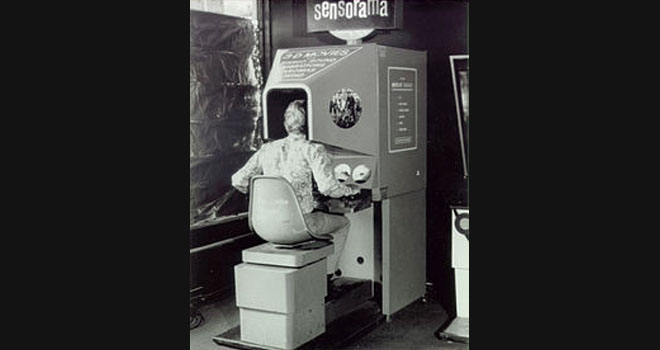
\includegraphics[width=0.75\textwidth]{sensorama-vr-machine.jpg}
\end{center}
\newpage \noindent
1960 veröffentlichte Heilig den ''Telesphere Mask'' welches das erste Head Mounted Display kurz HMD war. Es verfügte über die
Funktion der Ausgabe von 3D Bildern und hatte eine Stereo Ausgabe. Dieses gerät verfügte jedoch noch nicht über die Funktion der
Bewegungsverfolgung, welches mit dem Gerät ''Headsight'' von Ceomeau und Bryen zwei Philco Corporation Ingenieuren kam. Es
verfügte über die Funktion der Bewegungsverfolgung des Kopfes. Dieses Gerät wurde nicht als VR Brille verwendet, sondern für das
Militär entwickelt welches diese Technologie als fern Steuerung von Kameras in riskanten Kriegsregionen verwendete.\cite{virtualrealityhistory}\\
Ivan Sutherland welcher Informatiker im Jahre 1965 war, veröffentlichte ein Paper namens Ultimate Display. In diesem beschrieb er
das Computer Hardware die virtuelle Welt erstellen und in Echtzeit verwalten sollte. Sein
\href{http://worrydream.com/refs/Sutherland%20-%20The%20Ultimate%20Display.pdf}{Paper} welches er veröffentliche wird als der Bauplan 
von heutigen VR Brillen gesehen.\cite{virtualrealityhistory}\\
Ab diesem Zeitpunkt wurden die ersten HMD mit dem Fokus auf virtuelle Welten erfunden. Das Gerät ''The Sword
of Damacles'' welches im Jahre 1968 erschien, wurde trotz seiner Fähigkeit 3D Modelnetze abhängig von der Position des Benutzers
anzuzeigen, wegen seiner Größe und Notwendigkeit an einer Decke montiert zu sein nicht weiter als im Labor
entwickelt.\cite{virtualrealityhistory} \\
\begin{center}
    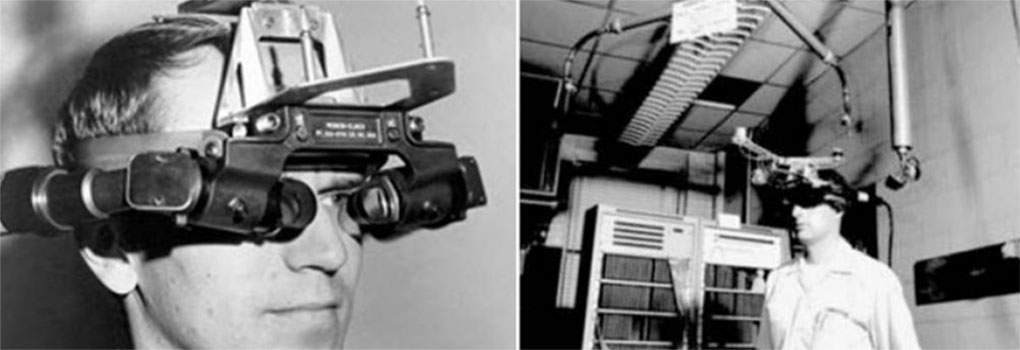
\includegraphics[width=0.75\textwidth]{sword-of-damacles.jpg}\cite{swordofdamacles}
\end{center}
Schon zu diesem Zeitpunkt experimentierte man damit, VR für Trainingsimulationen und Medizinischen Behandlungen zu verwenden. \\ 
Es wurde im Jahre 1979 von McDonnel-Douglas Corporation ein HMD für den militärischen Gebrauch entwickelt. Dieses Gerät war in der
Lage die Augen des Benutzers zu verfolgen um Bilder in Echtzeit passend zum Blickwinkel des Tragenden zu generieren.\cite{virtualrealityhistory}
\begin{center}
    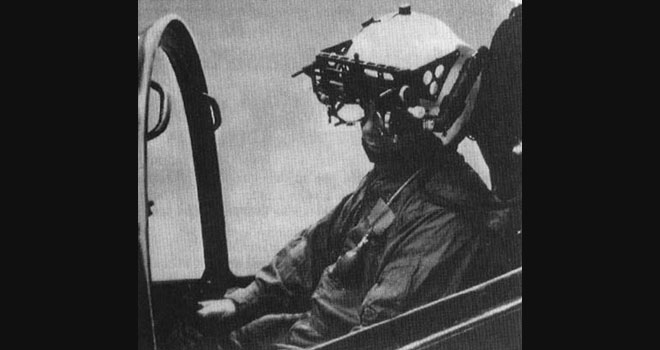
\includegraphics[width=0.5\textwidth]{VITAL-helmet-vr.jpg}\cite{vitalhelmet}
\end{center}
\newpage \noindent
Ebenso wurde im Jahre 1989 von der Nasa ein HMD entwickelt, um Astronauten anhand von VR Welten auszubilden.  
\begin{center}
    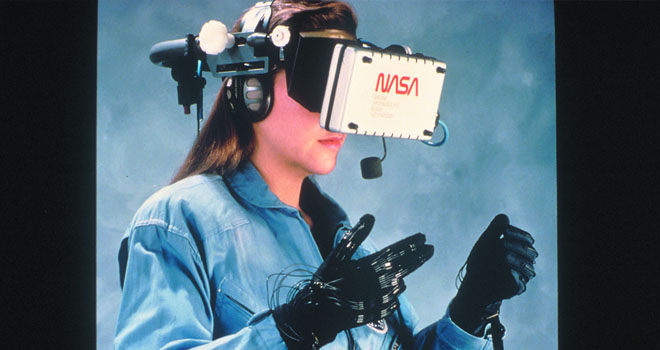
\includegraphics[width=0.5\textwidth]{virtual-environment-workstation-project-nasa.jpg}\cite{nasahelmet}
\end{center}
Einen Medizinischen gebraucht fand VR im Jahre 1997 durch die Georgia Tech und Emory University, welche den gebrauch von VR im
Posttraumatischen Belastungsstörungen für Veteranen erforschten. Hier wurden Kriegsszenarien simuliert welche Virtual Vietnam benannt. Diese
wurden verwendet um diese Symptome zu behandeln.\\ \\ 
Links zu Berichten die zu dieser Behandlung veröffentlicht wurden:
\begin{center}
    \href{http://gotz.web.unc.edu/files/2013/10/icat.pdf}{Virtual Vietnam}
    \href{http://gotz.web.unc.edu/files/2013/10/jts1999.pdf}{Virtual Reality Exposure Therapy for PTSD} \\
    \cite{virtualrealityhistory}
\end{center}
Jaron Lanier und Thomas Zimmerman, gründer von VPL Research Inc., waren die ersten die im Jahre 1985 VR Brillen und Handschuhe für die Masse
produzierten und verkauften. Hierauf folgte bis auf den internen Gebrauch von VR Technologien wie von der Nasa oder medizinischen
Experimenten bis zum Jahre 2010 nichts neues.\cite{virtualrealityhistory}\\ \\
Palmer Luckey, erzeugte den ersten Prototypen für die Oculus Rift welcher den Entwicklungsdrang von VR Technologien wieder neu entfachte.  
Folgen tut eine Kickstarter Kampanie im Jahre 2012 welche 2.4 Millionen USD sammelte und die Produktion der Oculus Rift Brillen
in gang brachte.\cite{virtualrealityhistory}\\
Heutzutage hat jeder Hersteller (HTC, Sony, Apple, Google, Amazon, Samsung) seine eigenen VR Brillen und der Markt und Gebrauch von VR
variiert von der Industrie, Medizien, Bildung, Unterhaltung bis hin zur Forschung.
\end{document}
